\documentclass[Space_Shuttle_Vessel_Manual.tex]{subfiles} 
\begin{document}

\section{MISSION CONFIGURATION}
\begin{multicols*}{2}
\label{sec:mission-configuration}
\renewcommand{\cfttoctitlefont}{\bf}
\localtableofcontents
\end{multicols*}

\begin{multicols*}{2}
\subsection{Overview}
\noindent
Space Shuttle Vessel uses a mission file to specify vehicle configuration and mission parameters. The mission files are in the JSON format, which allows manual editing, but they can be easily managed with the SSV Mission Editor. After a mission is defined, the Mission Editor can create a pre-launch scenario for that mission.\\
Mission files are declared as scenario file parameters for SSV vessels, by having the entry "MISSION" followed by the name of the mission file, and must be placed in the directory "<Orbiter installation>\textbackslash Missions\textbackslash SSV", or a sub folder.\\
The SSV installation already has some mission files for the included scenarios.


\newpage
\subsection{Mission Editor}
\noindent
The SSV Mission Editor allows the user to easily create and edit a mission file, and then to create scenarios for them. It is located in the <Orbiter installation>\textbackslash Utils folder.\\
The first time the Mission Editor is run it will ask for the location of the orbiter.exe file, so the Mission and Scenario folders can located.\\
The SSV Mission Editor work flow is as follows: create a new mission or open an existing mission, edit the mission parameters, save the mission file and, if desired, create a pre-launch scenario for that mission.\\
Several mission parameters aren't implemented yet in the vessels, but are already presented in the Mission Editor as they will be implemented in future versions.\\
The Mission Editor has the mission parameters grouped into tabs, which are detailed below.


\subsubsection{FLT NO tab}
Here the user can define the name of the mission, as well as a brief description of it.


\subsubsection{ORBITER tab}
OV configuration is defined in this tab. Name, texture and basic parameters such as Ku-band antenna can be configured here.
Custom OV textures must be located in folder "<Orbiter installation>\textbackslash Textures\textbackslash SSV\textbackslash OV".


\subsubsection{CREW MODULE tab}
This tab allows the user to define the configuration of the Crew Module.\\
None of these parameters are currently used, but are planned for a future version.


\subsubsection{LAUNCH tab}
This tab contains the controls to define launch site details and launch time.\\
Also in this tab is the Ascent Target calculator, which allows the user to define several ascent-related parameters, as well as a target orbit, for which MECO and OMS burn parameters will be calculated. Target altitudes for OMS-1 (Standard Insertion) or MECO (Direct Insertion), and OMS-2 can be defined, allowing both circular and elliptical orbits to be targeted. Target altitudes are input in Nautical Miles, and a conversion to Kilometers is shown in the tooltip of each text box.\\
After input parameter definition, the "Calculate" button initiates the required calculations to obtain the MECO and OMS burn parameters, after which orbital and burn information is shown. The "Save" button transfers the calculated MECO parameters to the Legacy MECO frame, and the OMS-1/2 parameters to the I-LOAD list.\\
The Ascent Target calculator currently do not take into account non-spherical gravity, so small errors will result if non-spherical gravity is enabled.\\
The Legacy MECO frame displays the MECO parameters for the mission. In a future version, these parameters will be replaced with a more correct implementation.\\
Currently, the Ascent Target calculator inputs are not saved.\\


\subsubsection{ORBIT tab}
Several maneuver sets for rendezvous orbit targeting are available for selection in this tab (custom parameters have to be manually configured in the I-LOADs tab). The orbital target vessel is also defined here.


\subsubsection{LANDING tab}
The Landing Site table is configurable in this tab, where the Runway database is displayed and runways can be chosen as primary or secondary runways in each of the Landing Site table entries.\\
The Landing Site table is displayed in a formatted way, to allow the user to save the list in a formatted copy.


\subsubsection{SSME tab}
Here the type of each SSME can be set.\\
None of these parameters are currently used (the SSMEs are all Block II), but are planned for a future version.


\subsubsection{CONSUMABLES tab}
OMS, RCS loads for all tanks are defined in this tab. The OMS Kit currently not implemented.\\
This tab also contains the settings to define the number of PDRS tank sets, EDO Kit and EDO pallets. The Dual EDO Pallet is currently not implemented.


\subsubsection{ET/SRB tab}
The type and parameters of the ET and SRBs are defined in this tab. In addition, custom textures can be also defined.\\
Custom ET textures must be located in folder "<Orbiter installation>\textbackslash Textures\textbackslash SSV\textbackslash ET", and custom SRB textures in the folder "<Orbiter installation>\textbackslash Textures\textbackslash SSV\textbackslash SRB".


\subsubsection{PAYLOAD tab}
The mission payloads are defined in this tab, and are grouped according to type.\\
At each payload location, the "Edit Payload" button allows the user to define the payload: vessel name, class, attachment ID and vessel-defined parameters (e.g., the payload might have solar panels that are folded during launch). Once the payload name is defined, it will be displayed to the right the controls.

\paragraph{Active and Passive Payloads}
For Active and Passive payloads, the "Edit Latches" button allows definition of latch parameters: number, location, orientation and their assignment to control systems, as well as the use of guides. A latch is enabled/disabled via a checkbox, and the button to its left allows the latch parameters to be edited. The button will show the PLID where the latch is installed, and it will be displayed in bold for the latch which represents the attachment.\\
To help visualize the location of the payload, a diagram of the payload bay (figure \ref{fig:plb_diagram}) is also shown, displaying valid locations for the latches as dark gray squares (and light gray squares for unavailable locations), as well as the current location of the current payload latches as colored rectangles: blue for the latch which represents the attachment, and green for the rest.\\
For Active payloads that are not present at launch (e.g., LDEF retrieval), the option exists to not define a payload.

\paragraph{Bay Bridge Payloads}
For Bay Bridge payloads, their bay and location is configurable.

\paragraph{Upper Stage Payloads}
One "Large Upper Stage" can be selected per mission: the Inertial Upper Stage (IUS), the Centaur G or the Centaur G-Prime. In addition, up to 3 "Small Upper Stages" can be selected per mission: the Payload Assist Module-A (PAM-A), PAM-D and PAM-D2. Currently no "Small Upper Stages" are available, but are planned for a future version. For each upper stage, configuration parameters and payload adapter parameters are also available.

\paragraph{Longeron Sill Payloads}
The RMS, MPM payloads such as the OBSS, and the SPDS, are also defined here.\\
Custom parameters for the RMS are available: CCTV camera details, and SN, which will only be used for display purposes in SPEC 94 (to be implemented in a future release).\\
The button "Use OBSS" sets the necessary parameters to install the OBSS in the Starboard MPM, while custom pedestal details can be defined for other payloads.\\
For the SPDS, the PRLA locations are configurable.\\
A payload can also be defined for the MPM Payload (optional) and SPDS (mandatory).\\
Currently the RMS and SPDS can only be on the port side, and the MPM Payload on the starboard side (other locations to be implemented in a future release).\\

\subsubsection{I-LOADs tab}
In this tab a list of the currently available I-LOADs is presented. These define various software parameters in the GPCs (e.g., SSME mission throttle setting).


\subsubsection{Test Mission}
The Test Mission button will run several checks to ensure everything is in order (e.g., each payload latch control system is only assigned to one payload latch).


\subsubsection{Create Scenario}
This button will open a new window to allow the user to create a scenario for the current mission. Several parameters are provided for editing before scenario generation.


\end{multicols*}

\begin{figure}[H]
	\centering
	\captionsetup{justification=centering}
  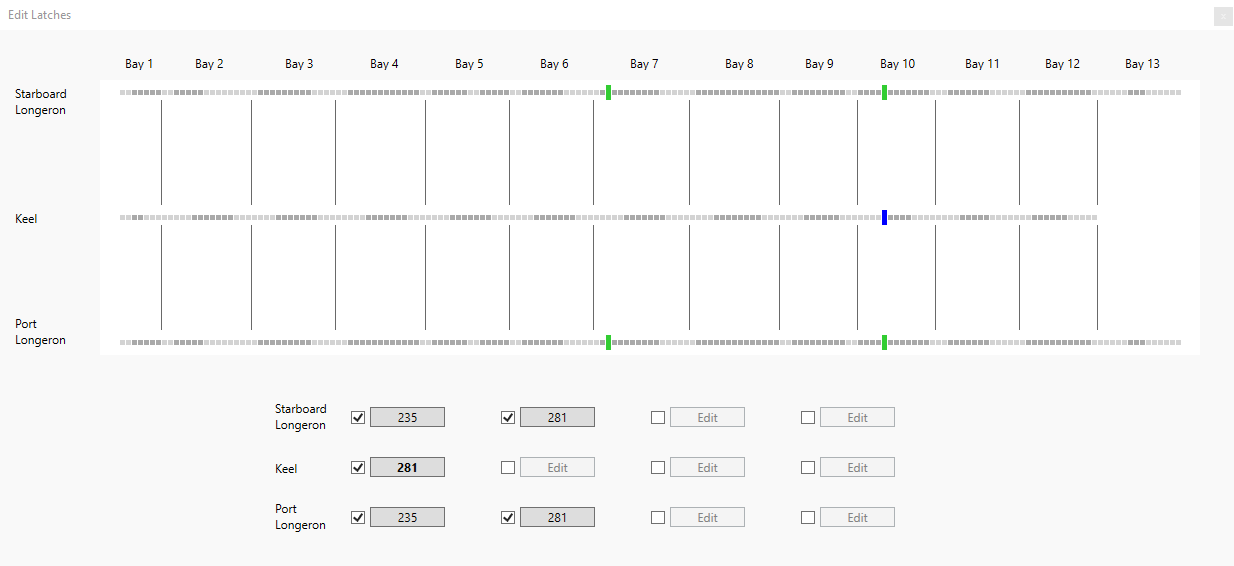
\includegraphics[width=0.99\hsize]{plb_diagram.png}
  \caption{Edit Latches window with payload bay diagram}
  \label{fig:plb_diagram}
\end{figure}

\end{document}
